
\section{Data Source and Task Definition}
\begin{figure}[htbp]
\centering
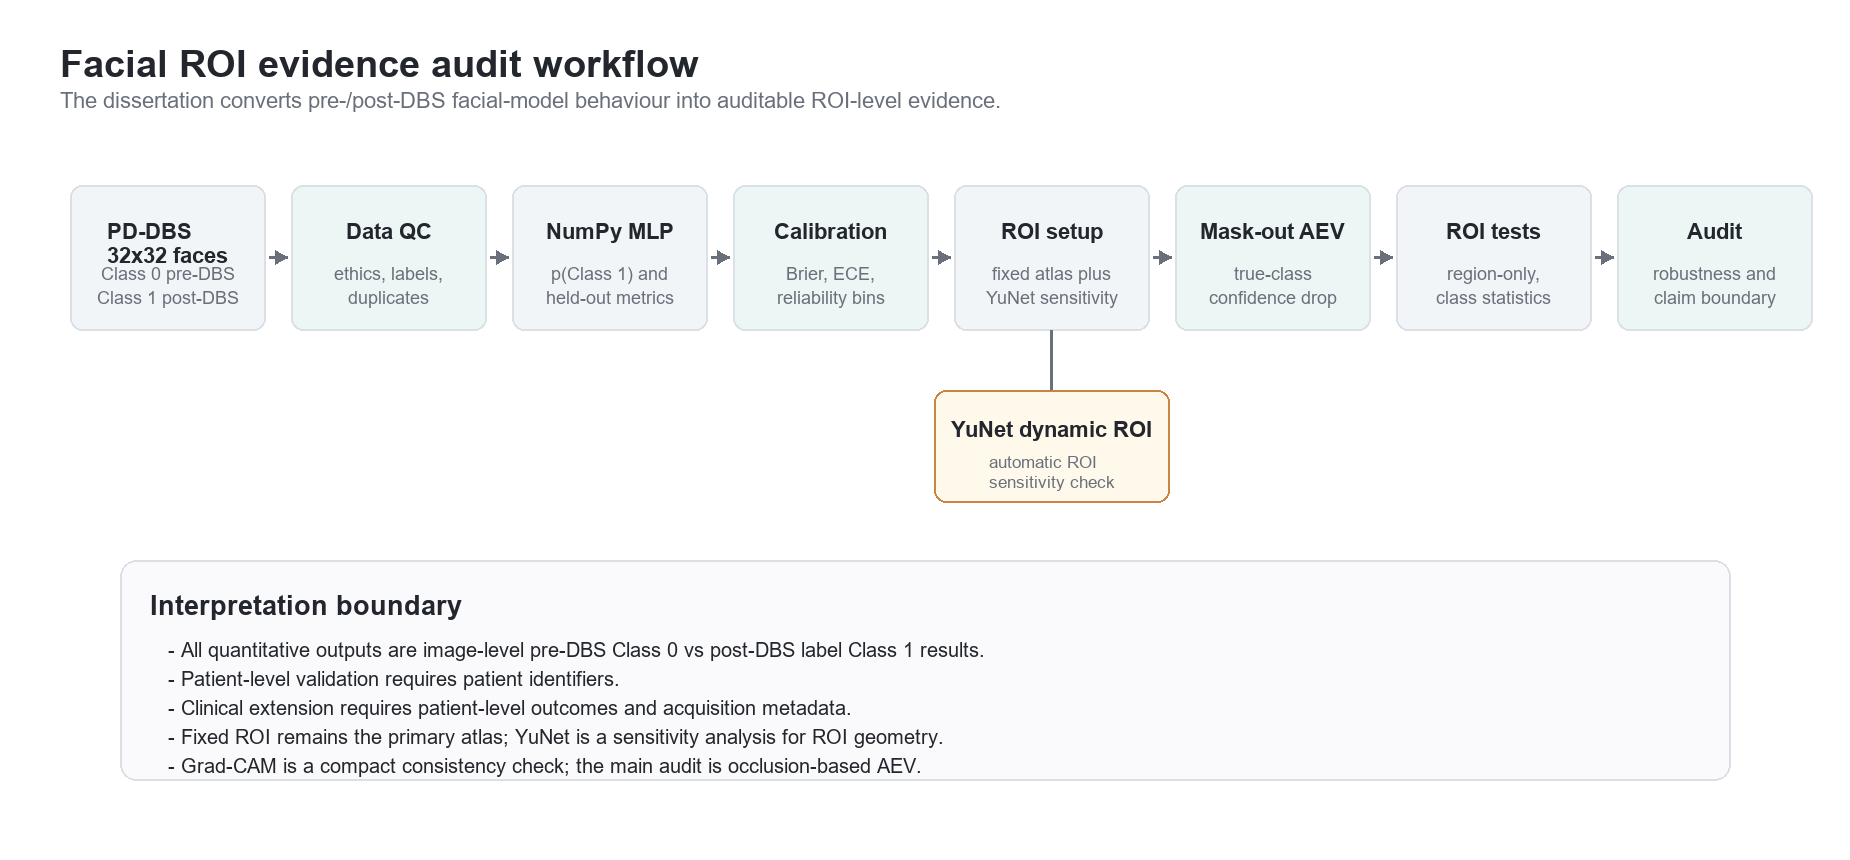
\includegraphics[width=0.98\textwidth]{figures/dissertation/fig_method_pipeline.png}
\caption{Facial ROI evidence audit workflow. The figure summarises the route from low-resolution PD-DBS facial images to pre-/post-DBS label classification, calibration, fixed and dynamic ROI definition, mask-out AEV, region-only validation, robustness checks, and explicit reporting scope.}
\end{figure}

The project used the local PD-DBS facial image file \path{data/raw/PD_DBS_Data.mat}. The file is a MATLAB 5.0 \path{.mat} file containing \texttt{\detokenize{x_train}}, \texttt{\detokenize{x_test}}, \texttt{\detokenize{y_train}}, and \texttt{\detokenize{y_test}}. It contains 2343 images in total: 1172 training images and 1171 test images.


The working file contained the image arrays and labels used for this study. Source-cohort details, acquisition protocol, original image resolution, down-sampling history, site or session variables, subject identifiers, and session identifiers were outside the provided metadata record. These fields were documented as study-scope variables and excluded from imputation.


Project ethics was approved by email after review of the submitted ethics form on 9 June 2026; the approval recorded that the dataset had already been authorised for research use.


Each image is represented as a 1024-dimensional vector corresponding to a 32$\times$32 grayscale image. Labels are encoded as 0/1 values under the project convention that Class 0 denotes pre-DBS and Class 1 denotes the supplied post-DBS label. All experiments therefore use the supplied pre-/post-DBS label task.


The provided record is image-level. The original train/test split was preserved to avoid introducing a new random split across all 2343 images. The supplied split is the reporting unit for all image-level experiments.


The task is therefore defined as a numeric binary classification problem. The classifier predicts the probability of Class 1, denoted \texttt{\detokenize{p_class1}}. The complementary probability for Class 0 is \texttt{\detokenize{1 - p_class1}}. This convention is used throughout baseline evaluation, calibration, occlusion, and AEV statistics.


\section{Data Loading and Quality Control (QC)}

A dedicated MATLAB 5 reader was implemented to keep data loading explicit and dependency-light. The loader extracts the four arrays, checks array dimensions, converts vectors to 32$\times$32 grayscale images, and preserves the original split. A contact sheet was generated to confirm that reconstructed images were visually interpretable as faces.


The raw image vectors were reshaped into 32$\times$32 images using the orientation chosen to match the visual structure observed in the original data-loading workflow. The reconstructed samples were inspected as a smoke test because an incorrect reshape order can transpose or distort faces.


The data QC stage recorded five key properties: total image count, split size, label counts, image resolution, and available metadata. These fields determine the reporting scope for the image-level pre-/post-DBS label experiments and explanation audits.


\section{Baseline Classification}

A compact NumPy multilayer perceptron (MLP) was used as the locked audit baseline to keep preprocessing, model fitting, prediction export, and downstream perturbation analysis reproducible within a small dependency footprint. A compact convolutional neural network (CNN) was trained separately as a secondary image model for architecture-sensitivity and Grad-CAM analysis.


The baseline uses per-feature z-score normalization fitted on the training subset, one hidden ReLU layer, a sigmoid Class 1 output, binary cross-entropy loss, and Adam-style optimization \boxcite{goodfellow2016deeplearning} \boxcite{kingma2015adam}. The original training set was split into training and validation subsets using stratification. The original test set was retained for final evaluation.


\begin{table}[htbp]
\centering
\scriptsize
\caption{NumPy MLP baseline specification}
\begin{tabularx}{\textwidth}{>{\raggedright\arraybackslash}X>{\raggedright\arraybackslash}X}
\toprule
Component & Specification \\
\midrule
Input & 1024 z-scored pixel values from each 32$\times$32 image \\
Architecture & One hidden ReLU layer with 64 units. Sigmoid Class 1 output \\
Loss and optimiser & Binary cross-entropy with Adam-style updates \\
Training protocol & Stratified 80/20 train/validation split within the supplied training set \\
Epochs and batch size & 300 epochs. Batch size 64 \\
Learning rate and L2 penalty & 0.001 learning rate. 0.0001 L2 penalty \\
Decision threshold & 0.5 on \texttt{\detokenize{p_class1}} for threshold metrics \\
Locked seed & 42 for the final headline run \\
\bottomrule
\end{tabularx}
\end{table}


Outputs use the fields \texttt{\detokenize{y_true}}, \texttt{\detokenize{p_class1}}, and \texttt{\detokenize{y_pred}}. The Class 1 probability is the supplied post-DBS label probability.


The locked MLP provides the saved probability outputs used for AEV, calibration, low-level, and region-only analyses. The compact CNN provides a second image-model check and the convolutional feature maps used for Grad-CAM.


Training used standard binary classification logic. The model was fitted on the training subset, monitored on a validation subset, and evaluated once on the held-out test split. Standardization parameters were fitted only from the training data and then applied to validation and test data. This avoids using test information during preprocessing. The final outputs include per-sample predictions so that later analyses can reuse the same probability values and avoid ad hoc retraining.


The evaluation metrics cover threshold-dependent and threshold-independent behaviour. Accuracy and F1 summarise performance at a classification threshold. Balanced accuracy accounts for class imbalance \boxcite{brodersen2010balanced}. AUROC assesses rank discrimination across thresholds \boxcite{fawcett2006roc}. Trapezoidal AUPRC summarises precision-recall behaviour when class proportions differ \boxcite{davis2006prroc} \boxcite{saito2015precision}. The majority-class baseline gives a simple reference for the imbalanced test set.


\section{Duplicate and Leakage QC}

Exact train-test duplicates were checked by hashing raw 1024-dimensional image vectors. Near-duplicate checks used nearest-train mean squared error (MSE) and maximum cosine similarity for each test image. This analysis can detect identical or highly similar images.


A second sensitivity analysis removed the flagged high-cosine near-duplicate test samples and recomputed key metrics. This check tests whether headline performance is dominated by a small number of duplicate or near-duplicate cases.


To assess broader similarity-related split sensitivity, an additional similarity-threshold analysis was added. The frozen test predictions were re-evaluated after excluding all test samples whose maximum cosine similarity to any training image exceeded progressively lower thresholds. This analysis is harsher than the original near-duplicate check because it removes broad similarity neighbourhoods.


Two low-level confound baselines were used. A global image-statistics baseline used eight non-anatomical summary features, including mean intensity, contrast, left-right mean difference, upper-lower mean difference, centre-border difference, and bright/dark pixel fractions. A per-ROI low-level baseline used five summary features per ROI: mean intensity, standard deviation, 10th percentile, 90th percentile, and mean gradient magnitude. These baselines assess how much label signal can be recovered from brightness, contrast, texture, and framing summaries without using the full pixel pattern.


The leakage and confound checks are therefore used as risk assessment. They document obvious duplicate leakage and provide context for the similarity-threshold and low-level baseline results.


\section{Calibration}

Calibration was evaluated from saved test-set predictions using Brier score and ECE with 10 equal-width bins over \texttt{\detokenize{p_class1}} \boxcite{brier1950verification} \boxcite{guo2017calibration}. Reliability-bin data were exported for later plotting.


The Brier score was computed as the mean squared error between predicted Class 1 probability and the numeric binary outcome. ECE was computed by assigning predictions to probability bins, calculating the absolute difference between mean confidence and observed Class 1 fraction in each bin, and taking the count-weighted average. Reliability-bin data were used to plot the observed Class 1 fraction against mean predicted probability.


The final reported calibration analysis uses the unscaled test-set probabilities from the locked baseline run \boxcite{guo2017calibration}. This documents the calibration context for the probability outputs used by AEV on the supplied pre-/post-DBS label task.


\section{Coarse Fixed-Atlas ROI Definition}

Eight mutually exclusive coarse named ROIs were defined on the 32$\times$32 image grid. The table below gives the intended facial-region scope and grid coverage for each region. Rows and columns use zero-indexed inclusive ranges. The machine-readable ROI names are stored in \path{outputs/roi/coarse_roi_definitions.csv}.


\begin{table}[htbp]
\centering
\scriptsize
\caption{Coarse fixed-atlas ROI definitions}
\begin{tabularx}{\textwidth}{>{\raggedright\arraybackslash}X>{\raggedright\arraybackslash}X>{\raggedright\arraybackslash}X>{\raggedright\arraybackslash}X>{\raggedright\arraybackslash}X}
\toprule
ROI & Anatomical coverage & Grid rows & Grid columns & Pixels \\
\midrule
Upper brow/forehead & Upper face, brow, forehead & 0-7 & 4-27 & 192 \\
Left periocular & Image-left periocular region & 8-14 & 0-13 & 98 \\
Right periocular & Image-right periocular region & 8-14 & 18-31 & 98 \\
Nasal midface & Nasal bridge and central midface & 8-21 & 14-17 & 56 \\
Left cheek/zygomatic & Image-left cheek and zygomatic region & 15-23 & 0-13 & 126 \\
Right cheek/zygomatic & Image-right cheek and zygomatic region & 15-23 & 18-31 & 126 \\
Perioral/mouth & Perioral and mouth region & 24-27 & 8-23 & 64 \\
Chin/mandible & Chin and mandible region & 28-31 & 6-25 & 80 \\
\bottomrule
\end{tabularx}
\end{table}

This coarse ROI design was used because the available image resolution supports broad region analysis. Standard facial landmark and face-localisation approaches assume substantially richer spatial detail than the present 32$\times$32 arrays provide \boxcite{kazemi2014one} \boxcite{zhang2016mtcnn} \boxcite{bulat2017far} \boxcite{deng2020retinaface}.


The ROI definitions were implemented as binary masks on the 32$\times$32 grid. Each mask identifies the pixels belonging to one named region. The masks were designed to be mutually exclusive, meaning that no pixel belongs to more than one ROI. This matters for interpretation: if ROIs overlap, evidence assigned to one region may partly duplicate evidence assigned to another. The final masks have zero overlapping pixels.


The fixed pixel-rectangle masks assume approximate face centring and similar framing. The provided record contained no landmark metadata, so centring was checked at a coarse level. Intensity-threshold foreground masks were used to estimate image centroids, bounding-box widths, bounding-box heights, and foreground fractions across train and test splits. This alignment QC summarises how the fixed-ROI layout matches the supplied 32$\times$32 images.


An automatic ROI-definition sensitivity analysis was added using OpenCV YuNet, a lightweight face detector designed for efficient face localisation \boxcite{wu2023yunet}. The original 32$\times$32 grayscale images were upsampled to 256$\times$256, YuNet detected the face and five coarse landmarks, and dynamic ROI boxes were derived to approximate the same eight ROI names. The primary AEV statistics used the fixed atlas so that every image shared one reproducible low-resolution coordinate system. YuNet was used to test how region-only and AEV results changed when ROI boxes followed detected face geometry.


\section{Occlusion-Based AEV}

For each test image and ROI, pixels inside the ROI were replaced by the corresponding training-set mean pixel values. The model then recomputed \texttt{\detokenize{p_class1}}.


True-class confidence was defined as:


\begin{verbatim}
true_confidence = p_class1       if y_true = 1
true_confidence = 1 - p_class1   if y_true = 0
\end{verbatim}

Occlusion evidence, reported as the true-class confidence drop, was defined as:


\begin{verbatim}
evidence_drop = true_confidence_original - true_confidence_masked
\end{verbatim}

Positive values indicate that masking the ROI reduced true-class confidence. The AEV for each image is the vector of true-class confidence drops across the eight ROIs.

\begin{figure}[H]
\centering
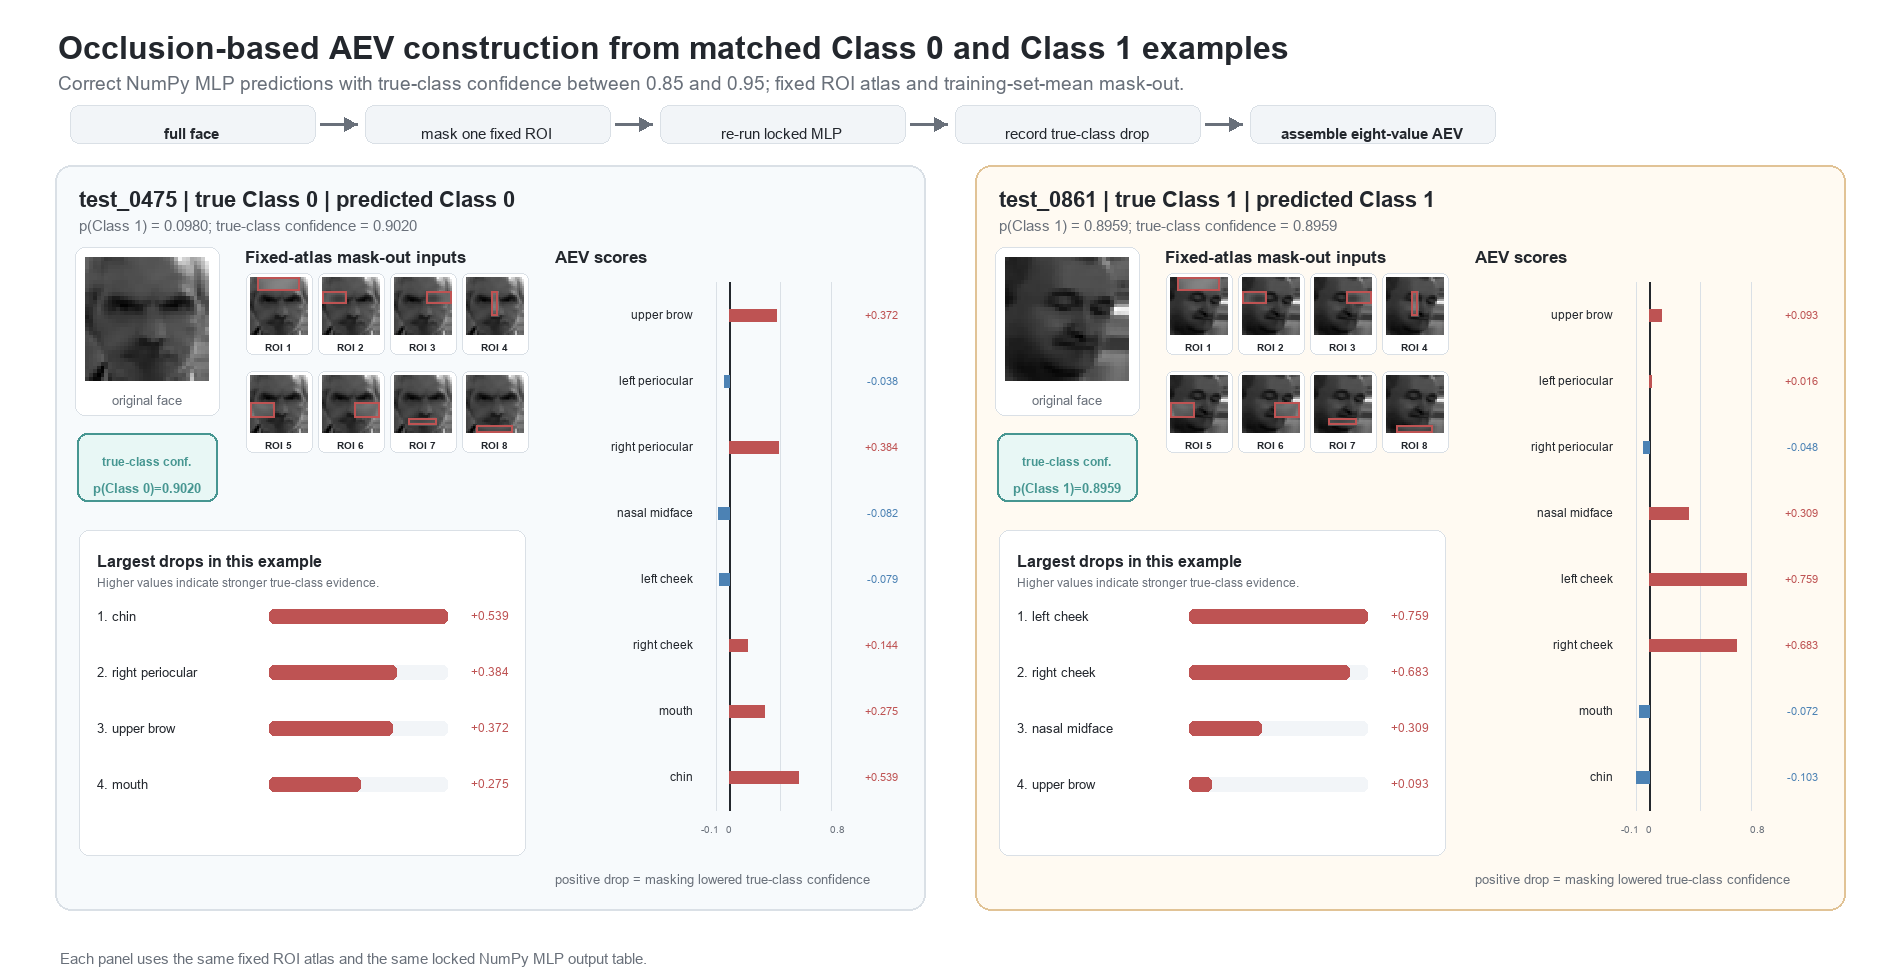
\includegraphics[width=\textwidth]{figures/dissertation/fig_aev_dual_worked_example.png}
\caption{Occlusion-based AEV construction for matched Class 0 and Class 1 test examples. Both examples are correct NumPy MLP predictions with true-class confidence between 0.85 and 0.95. For each sample, the figure shows the original 32$\times$32 face, eight fixed-atlas ROI mask-out inputs, and the resulting true-class confidence-drop vector.}
\end{figure}


The word anatomical is used operationally: it refers to the named coarse ROI coordinate system on the 32$\times$32 image grid. This convention keeps AEV scores tied to the implemented ROI layout.


Using the training-set mean as the replacement value avoids introducing an extreme artificial colour or intensity patch. It creates a neutralised version of the region relative to the learned training distribution. The perturbed image is still artificial, and attribution results can depend on the chosen baseline or reference value. The choice is a standard and transparent perturbation baseline for a low-resolution study \boxcite{zeiler2014visualizing} \boxcite{samek2017evaluating} \boxcite{sturmfels2020baselines}.


The use of true-class confidence is also deliberate. For correctly classified samples, true-class confidence and predicted-class confidence are usually the same. For misclassified samples, the two values differ. True-class drop measures how much masking a region reduces confidence in the ground-truth numeric label, including misclassified samples.


For each image, the final AEV is:


\begin{verbatim}
AEV_i = [drop_upper_brow_forehead, drop_left_periocular,
         drop_right_periocular, drop_nasal_midface,
         drop_left_cheek_zygomatic, drop_right_cheek_zygomatic,
         drop_perioral_mouth, drop_chin_mandible]
\end{verbatim}

Each component can be analysed per image, averaged across samples, compared between classes, or ranked within perturbation experiments.


\section{AEV Size Sensitivity}

Fixed-atlas mask-out scores were also summarised after dividing each ROI's mean true-class confidence drop by its pixel count. The normalized value was reported as confidence drop per 100 pixels:


\begin{verbatim}
drop_per_100_pixels = 100 * mean_evidence_drop / ROI_pixel_count
\end{verbatim}

This analysis checks how strongly raw full-region mask-out rankings track ROI size. Because raw mask-out drops scale with the number of masked pixels, cross-ROI comparisons of evidence intensity use the size-normalized score (confidence drop per 100 pixels) as the primary ranking lens. The raw AEV score is retained as the measure of the total effect of masking a complete named region. Both are reported so that total-region contribution and size-adjusted intensity can be read side by side.


\section{AEV Statistics}

Class 0 and Class 1 AEV distributions were compared ROI by ROI. The analysis computed class means and medians, mean difference, Cohen's d, Cliff's delta, permutation-test p-values, Benjamini-Hochberg FDR-adjusted p-values, and bootstrap 95\% confidence intervals \boxcite{cohen1988statistical} \boxcite{cliff1993dominance} \boxcite{benjamini1995controlling} \boxcite{efron1993bootstrap}.


The mean difference was defined as Class 1 mean evidence minus Class 0 mean evidence. A positive difference therefore indicates higher evidence in Class 1. A negative difference indicates higher evidence in Class 0. This convention is used consistently in the class-specific figures and tables.


Permutation testing was used because it makes fewer distributional assumptions than a parametric test \boxcite{good2005permutation}. For each ROI, class labels were repeatedly shuffled and the observed mean difference was compared against the null distribution of permuted differences. FDR correction was applied across the eight ROI tests to control false discovery rate. Effect sizes were reported because p-values alone leave the magnitude of regional evidence differences unspecified.


Bootstrap confidence intervals quantified uncertainty in the estimated mean differences.

The class-specific AEV analysis was run on the supplied test split used for the main fixed-split benchmark. The analysis used the same ROI masks, MLP probabilities, fill rule, confidence-drop definition, permutation testing, FDR correction, and bootstrap interval procedure for all eight ROIs.


\section{ROI Low-Level Confound Baseline}

The per-ROI low-level confound baseline was trained on 40 scalar features extracted from the same eight fixed ROIs. The feature set contained five summaries for each ROI: mean intensity, standard deviation, lower and upper intensity percentiles, and mean local gradient magnitude. The baseline used a standardised linear probabilistic classifier with the supplied train/test split.


This experiment tests whether broad ROI-local intensity and texture summaries carry label information. It uses summary-level regional features as a low-level comparator for AEV, raw-pixel modelling, and region-mask perturbation results.


\section{Pixel-Occlusion XAI Baseline}

As an additional explanation baseline, each pixel was occluded individually by replacing it with its training-set mean value. The true-class confidence drop for each pixel was then aggregated into the same eight fixed ROIs. This pixel-level baseline perturbs one pixel at a time before ROI aggregation. Region-mask AEV masks a complete region in one perturbation.


The pixel-occlusion baseline was compared with region-mask AEV using Spearman ROI-rank correlation and top-three ROI overlap. This provided a lightweight XAI comparator using the same trained MLP, test set, labels, fill value, and ROI atlas.


\section{Region-Only Validation}

For each ROI, pixels inside the ROI were retained and all other pixels were replaced with training-set mean values. The classifier then generated predictions from the region-only image. This measured retained-region response under the fixed MLP.


Region-only validation complements mask-out AEV. A high mask-out drop indicates that a region supports the full-face model in context. A high region-only AUROC indicates that the region alone contains information that can rank the numeric classes. Because facial evidence is likely distributed, region-only performance is expected to be lower than full-face performance. The key question is whether any region performs above chance or majority baseline.


The region-only experiment used the same trained MLP and the same test set. Differences across ROIs therefore reflect input perturbation under fixed model weights. Metrics were computed for each ROI separately, including accuracy, balanced accuracy, AUROC, trapezoidal AUPRC, and mean true-class confidence.


\section{Robustness}

Robustness analyses included near-duplicate sensitivity, five-seed training stability, mild blur perturbation, crop/resize perturbation, ROI evidence ranking stability under perturbation, fixed-ROI jitter, YuNet multi-seed checks, bootstrap fixed-versus-YuNet comparisons, label permutation, and occlusion fill-strategy sensitivity.


Multi-seed robustness was assessed across repeated random validation splits and model initialisations. This test captures variability from seed-dependent validation sampling and training, and the results are summarised as mean, standard deviation, and range across runs.


Perturbation robustness tested whether the trained model and the ROI evidence pattern were sensitive to small image changes, following the broader idea that vision models should be stress-tested under common corruptions and perturbations \boxcite{hendrycks2019robustness}. Mild blur approximates loss of sharpness. Centre crop and offset crop approximate spatial framing changes. At 32$\times$32 resolution, crop-based perturbations can shift or remove a large fraction of the face. For ROI evidence stability, rank correlation and top-3 overlap were used to assess whether high-evidence regions remained high under perturbation.


\section{Compact CNN and Grad-CAM Consistency Check}

The main audit pipeline used locked MLP probabilities for occlusion-based AEV, giving ROI-level evidence scores from one reproducible probability source. A compact PyTorch CNN was trained as a secondary image model for architecture-sensitivity and Grad-CAM analysis. Occlusion-based AEV uses forward passes through the MLP. Grad-CAM is computed from the CNN's convolutional feature maps. Cross-model agreement is reported as architecture-sensitivity evidence across model class and explanation mechanism. True-class Grad-CAM heatmaps were generated from the CNN and projected into the same eight fixed ROI masks used for occlusion \boxcite{zhou2016cam} \boxcite{selvaraju2017gradcam}.


Agreement was assessed at two levels. First, ROI-level Grad-CAM energy fractions were ranked against same-CNN ROI mask-out evidence drops using Spearman rank correlation and top-k ROI overlap. Second, a mean Grad-CAM map was compared with the ROI-weighted occlusion map using pixel top-k overlap. This check measures whether a gradient-based CNN explanation broadly supports the same regional evidence pattern as functional ROI occlusion.

Cross-model MLP-AEV/CNN-Grad-CAM comparisons were reported as sensitivity comparisons, with model architecture and explanation mechanism both changing.


\section{Controlled Comparison and Sensitivity Design}

The experiments were organised so that each comparison had a defined control structure. Same-model and same-split analyses were treated as controlled comparisons. Analyses that changed the split, ROI geometry, sample set, or model architecture were reported as sensitivity analyses, stress tests, or consistency checks.


\begin{table}[htbp]
\centering
\scriptsize
\caption{Controlled comparison design summary}
\begin{tabularx}{\textwidth}{>{\raggedright\arraybackslash}X>{\raggedright\arraybackslash}X>{\raggedright\arraybackslash}X>{\raggedright\arraybackslash}X}
\toprule
Experiment & Held constant & Changed or tested & Role in the audit \\
\midrule
Baseline MLP & Supplied train/test split, labels, preprocessing rule, threshold reporting & Learned numeric classifier & Establishes the predictive substrate for later explanation tests \\
Calibration & Saved MLP test predictions and supplied test labels & Probability bin and calibration metric & Checks whether confidence values used by AEV are numerically interpretable \\
Fixed-atlas mask-out AEV & MLP weights, test set, labels, fill value, eight fixed ROI names & Masked ROI & Controlled perturbation test of full-region contribution \\
Class-specific AEV statistics & Same AEV table, same test split, same ROI definitions & Class group comparison & Tests whether regional evidence differs between Class 0 and Class 1 \\
ROI low-level confound baseline & Same fixed ROI names and supplied split & ROI-local intensity and texture summaries & Assesses low-level regional confound signal without raw pixel-pattern modelling \\
Pixel-occlusion baseline & Same MLP, test set, labels, fill value, and ROI atlas & Pixel-wise occlusion followed by ROI aggregation & Provides a lightweight XAI comparator for region-mask AEV \\
Region-only validation & Same MLP, same test set, same fill value, same metric definitions & Retained ROI & Tests whether individual regions contain independent signal \\
Fixed atlas versus YuNet ROI & Same MLP, test set, labels, fill value, and ROI names & ROI geometry and pixel count & ROI-definition sensitivity analysis \\
Robustness checks & Frozen metrics or repeated training protocol, depending on test & Seed, blur, crop, fill value, label permutation, or ROI jitter & Stability and failure-mode assessment \\
Compact CNN / Grad-CAM & Same CNN, same test split, same true-class target & Explanation view and ROI projection & Secondary image-model and explanation-consistency check \\
\bottomrule
\end{tabularx}
\end{table}

This design assigns each result a defined evidential role. The main AEV and region-only analyses are controlled perturbation experiments under fixed model weights. YuNet and ROI jitter test sensitivity to ROI geometry. Low-level global and ROI baselines test brightness, texture, and framing signal. The reported values come from staged scripts and machine-readable outputs under \path{outputs/} and \path{models/}.


